\chapter{Oscillation Probability Calculation}
\label{chap:OscillationProbability}

\section{Overview}
\label{sec:Oscillation_Overview}

The analysis presented within this thesis focuses on the determination of oscillation parameters from atmospheric and beam neutrinos. Whilst subject to the same oscillation probability, the way in which the two sets of samples have sensitivity to the different oscillation parameters differs quite significantly.

Atmospheric neutrinos have a varying baseline such that the distance each neutrino travels before interacting is dependent upon the zenith angle. Therefore the oscillation probability can be represented as a two-dimensional ``oscillogram'' as shown in \autoref{fig:Oscillation_SK_BasicOscillogram}. For this calculation, four layers of fixed density were used to model the Earth with values taken from an approximation of the PREM model. The oscillogram shows the different layers and how the oscillation probability reacts to them (The fourth layer, 'inner core', is very close to \quickmath{cos(\theta_{Z}) = -1.0 and is not visible}). \finish{I don't know if I trust this}.

\begin{figure}[h]
  \begin{subfigure}[t]{0.8\textwidth}
    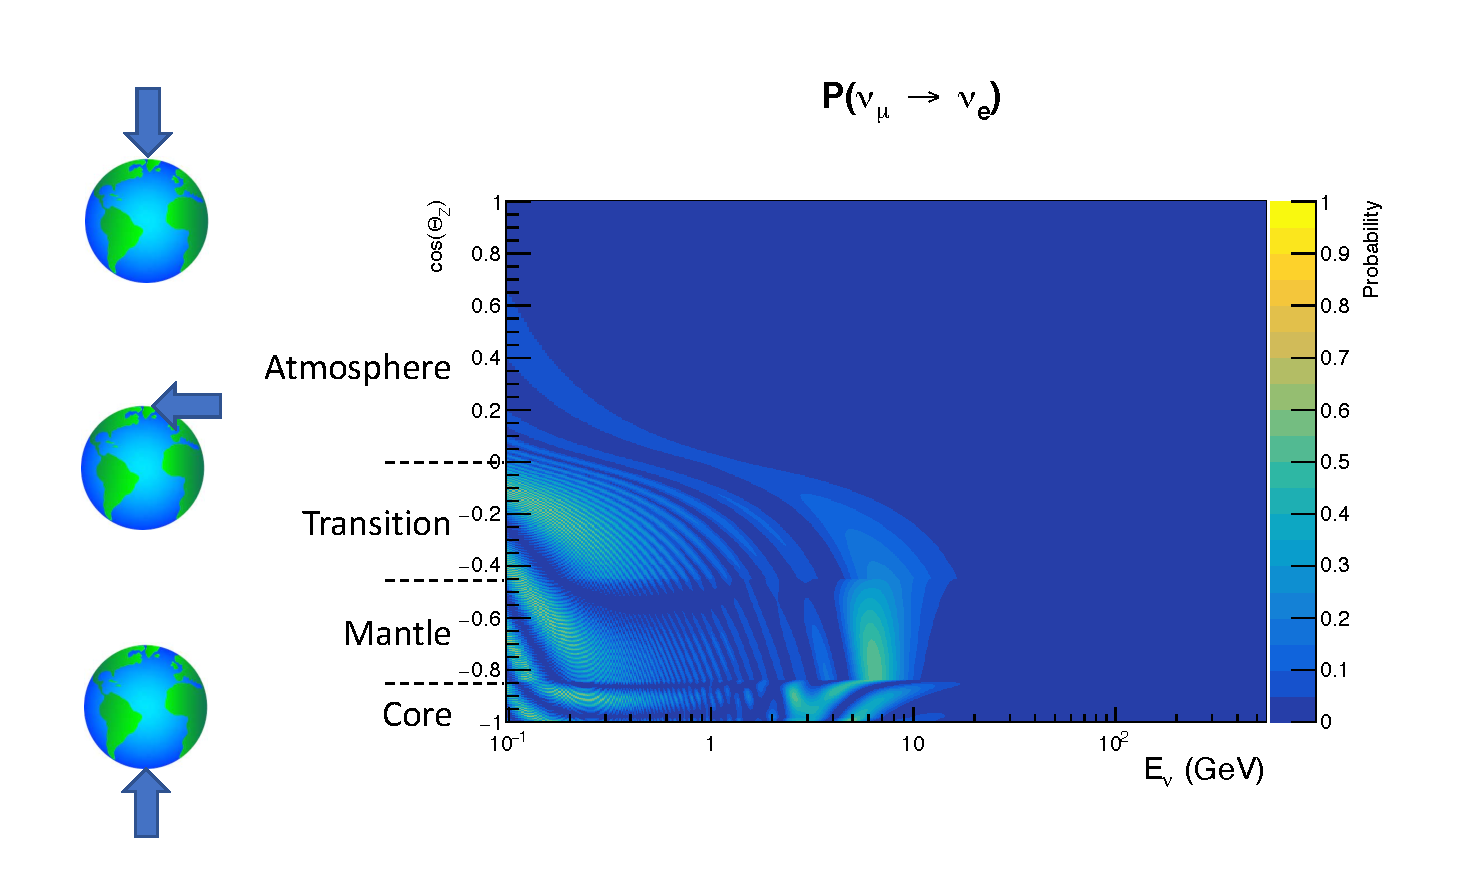
\includegraphics[width=\textwidth, trim={0mm 0mm 0mm 0mm}, clip,page=1]{Figures/Oscillation/BasicOscillogramWithNotes.pdf}
  \end{subfigure}
  \caption{An ``Oscillogram'' that depicts the \quickmath{P(\nu_\mu \rightarrow \nu_e)} oscillation probability as a function of neutrino energy and cosine of the zenith angle. The zenith angle is defined such that \quickmath{\cos(\Theta_{Z}) = 1.0} represents neutrinos which travel from directly above the detector. The four layer constant density PREM model approximation is used and Asimov A oscillation parameters are assumed.}
  \label{fig:Oscillation_SK_BasicOscillogram}
\end{figure}

Atmospheric neutrinos do have some sensitivity to \dcp through a normalisation term. \autoref{fig:Oscillation_SK_DCPSensitivity} illustrates the difference in oscillation probability between CP-conserving and CP-violating \dcp values. The result is a complicated oscillation patter in the appearance probability for sub-GeV upgoing neutrinos. The detector does not have sufficient resolution to resolve these individual patterns so the sensitivity to \dcp for atmospheric neutrinos comes via the overall normalisation of the sub-GeV upgoing events. The presence of matter means that the effect \dcp has on the oscillation probability is not equal between neutrinos and antineutrinos which would be expected in vacuum. This is further extenuated by the fact that SK can not distinguish neutrinos and antineutrinos well and that the cross section neutrino interaction is larger than that for antineutrinos. Finally, sample selections (discussed in \finish{Link to selection chapter}) targeting different neutrino interactions modes (charge current quasi-elastic and single pion production) result in an inbalance in the percentage of neutrinos to anti-neutrinos in these samples due to pion capture. Negatively charged pions from antineutrino interactions are more likely to be captured by a nucleus compared to a positively charged pion emitted from a neutrino interaction. This all culminates in atmospheric neutrinos having a very complex sensitivity to \dcp.

\begin{figure}[h]
  \begin{subfigure}[t]{0.8\textwidth}
    \includegraphics[width=\textwidth, trim={0mm 0mm 0mm 0mm}, clip,page=1]{Figures/Oscillation/AtmDCPSens.pdf}
  \end{subfigure}
  \caption{}
  \label{fig:Oscillation_SK_DCPSensitivity}
\end{figure}

Atmospheric neutrinos are subject to matter effects as they travel through the dense matter in the Earth. The vacuum and matter oscillation probabilities for \quickmath{P(\nu_{e} \rightarrow \nu_{e})} and \quickmath{P(\bar{\nu}_{e} \rightarrow \bar{\nu}_{e})} are presented in \autoref{fig:Oscillation_SK_VacuumMatter}. The oscillation probabilty for both neutrinos and antineutrinos are effected in the preresence of matter but the resonance (Effects around \quickmath{E_{\nu} \sim 5\teext{GeV}}) only occurs for neutrinos in normal mass hierarchy and antineutrinos for inverse mass ordering. The exact position and amplitude of the resonance depends on both \sinsqatm meaning that the atmospheric neutrinos have sensitivity to the octant of \quickmath{\theta_{23}}. The matter resonance only occurs 

\begin{figure}[h]
  \begin{subfigure}[t]{0.8\textwidth}
    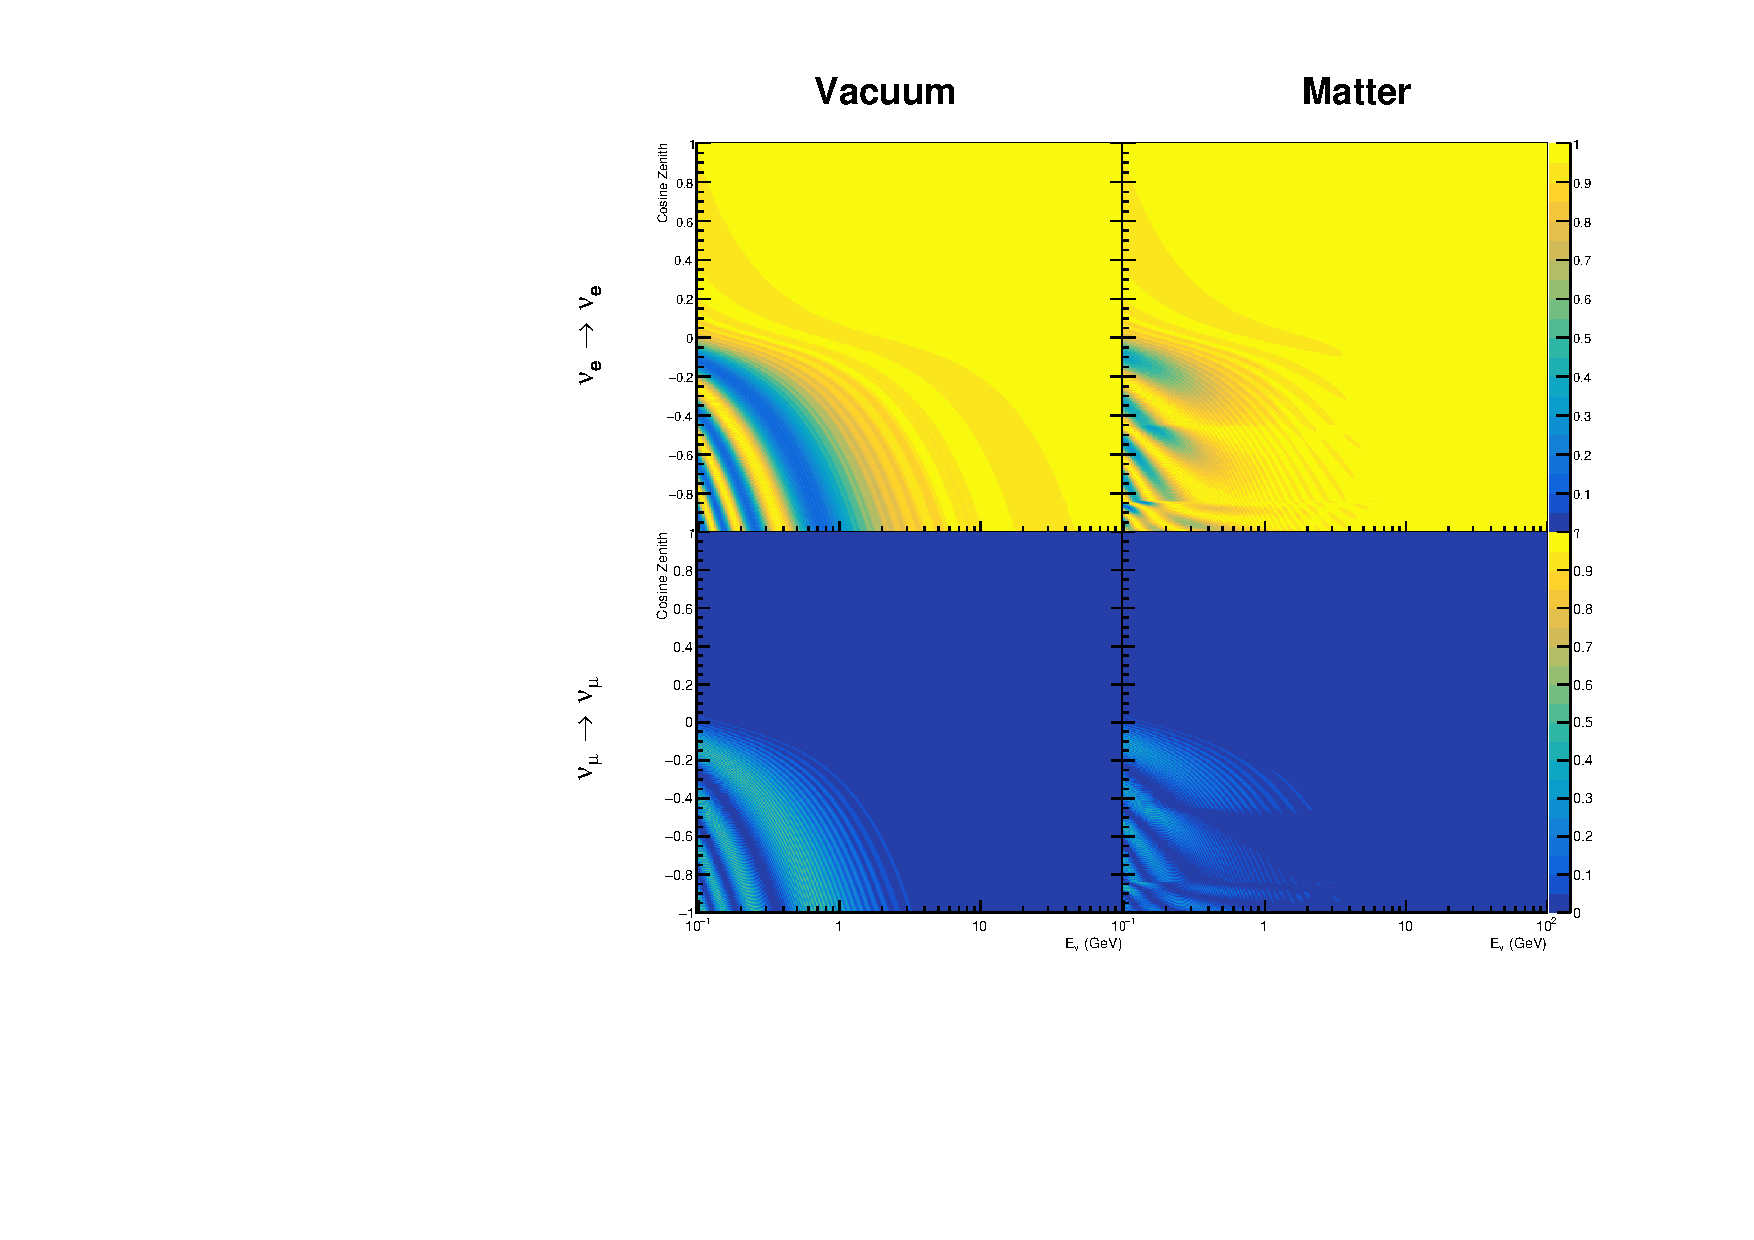
\includegraphics[width=\textwidth, trim={0mm 0mm 0mm 0mm}, clip,page=1]{Figures/Oscillation/MatterEffect.pdf}
  \end{subfigure}
  \caption{}
  \label{fig:Oscillation_SK_VacuumMatter}
\end{figure}

As the T2K beam flux is centered at the first oscillation maximum, the sensitivity to \dcp is predominanetly observed as a change in the event-rate of e-like samples in \quickmath{\nu/\bar{\nu}} modes. \autoref{fig:Oscillation_T2K_OscillationProbSensitivity} illustrates the \quickmath{P(\nu_\mu \rightarrow \nu_e)} oscillation probability for a range of \dcp values. %The magnitude of the oscillation peak has an approximate factor of two difference between the CP-violating values \quickmath{\delta_{CP} = \pm\pi/2} and the difference in oscillation probability between the CP-conserving
A circular modulation of the oscillation peak (in both magnitude and position) is observed when varying throughout the allowable values of \dcp. The CP-covserving values of \quickmath{\delta_{CP}=0,\pi} have a lower(higher) oscillation maximum than the CP-violating values of \quickmath{\delta_{CP}=-\pi/2}(\quickmath{\delta_{CP}=\pi/2}) leading to a \quickmath{\sin{\delta_{CP}}} type sensitivity. A sub-dominant shift in the energy of the oscillation peak is also present to aid separating the two CP-conserving value of \dcp.

T2K's sensitivity to the atmospheric oscillation parameters is more of a shape-based variation of the muon-like samples, as illusrated in \autoref{fig:Oscillation_T2K_OscillationProbSensitivity}. The value of \quickmath{\Delta m^{2}_{32}} laterally shifts the position of the oscillation dip (around \quickmath{E_\nu \sim 0.6\text{GeV}}) in the \quickmath{P(\nu_\mu \rightarrow \nu_\mu)} oscillation probability. The variation of \sinsqatm is not as straight-foward to interpret due to matter effects. The predominant effect is to vertically shift the oscillation dip but matter effects also induce second order terms to laterally shift the position of the dip.

\begin{figure}[h]
  \begin{subfigure}[t]{0.5\textwidth}
    \includegraphics[width=\textwidth, trim={0mm 0mm 0mm 0mm}, clip,page=1]{Figures/Oscillation/T2K_NuMu_x_NuMu_DelMsq32Sens.pdf}
    \subcaption{\delmsqatm}
  \end{subfigure}%
  \begin{subfigure}[t]{0.5\textwidth}
    \includegraphics[width=\textwidth, trim={0mm 0mm 0mm 0mm}, clip,page=1]{Figures/Oscillation/T2K_NuMu_x_NuMu_Sinsqth23Sens.pdf}
    \subcaption{\sinsqatm}
  \end{subfigure}
  \begin{subfigure}[t]{0.5\textwidth}
    \includegraphics[width=\textwidth, trim={0mm 0mm 0mm 0mm}, clip,page=1]{Figures/Oscillation/T2K_NuMu_x_NuE_DCPSens.pdf}
    \subcaption{\dcp}
  \end{subfigure}
  \caption{}
  \label{fig:Oscillation_T2K_OscillationProbSensitivity}
\end{figure}

To allow comparisons between the joint analysis and the single experiment analyses, two sets of oscillation parameters have been defined.

\begin{table}[ht!]
    \centering
    \begin{tabular}{c|c|c}
      \hline
      \hline
      Parameter & Asimov A & Asimov B \\
      \hline
      \quickmath{\Delta m^{2}_{12}} & \multicolumn{2}{c}{\quickmath{7.53 \times 10^{-5} \text{eV}^{2}}} \\ \hline
      \quickmath{\Delta m^{2}_{32}} & \multicolumn{2}{c}{\quickmath{2.509 \times 10^{-3} \text{eV}^{2}}} \\ \hline
      \quickmath{\sin^{2}\left(\theta_{12}\right)} & \multicolumn{2}{c}{\quickmath{0.304}} \\ \hline
      \quickmath{\sin^{2}\left(\theta_{13}\right)} & \multicolumn{2}{c}{\quickmath{0.0219}} \\ \hline
      \quickmath{\sin^{2}\left(\theta_{23}\right)} & \quickmath{0.528} & \quickmath{0.45} \\ \hline
      \quickmath{\delta_{CP}} & \quickmath{-1.601} & \quickmath{0.0} \\ \hline
      \hline
    \end{tabular}
    \caption{}
    \label{tab:Oscillation_ParameterSets}
\end{table}
